\chapter*{Introducere} 
\addcontentsline{toc}{chapter}{Introducere}

\section*{Context}
\addcontentsline{toc}{section}{Context}

Știință și tehnologie.
Acest duo se regăsește la orice pas al secolului XXI și interacționăm cu el zilnic, mai mult sau mai puțin, prin intermediul multor dispozitive precum telefonul, televizorul sau calculatorul personal.
Într-o formă sau alta, dispozitivele de acest fel (\emph{împreună} cu mulțimea de aplicații software pe care le rulează) fac lumea mai \emph{accesibilă} pentru utilizatorii lor – de pildă, să verificăm vremea zilei de mâine pe un laptop sau să ne bazăm pe comenzile online în timpul unei pandemii.
Astfel de exemple ne arată cum tehnologia modelează felul în care ne desfășurăm activitățile zilnice și ``scurtăturile'' pe care le putem lua pentru a îndeplini anumite sarcini – desigur, în anumite cazuri, cu niște costuri aferente.

În paragraful de mai sus este accentuat termenul ``accesibil'' care, prin definiție\footnote{Definiție preluată din DEX 2009}, înseamnă ceva ``care este la îndemâna cuiva; care poate fi ușor procurat''.
Am văzut cum lumea poate fi ``mai la îndemâna cuiva'' – dar cum facem ca tehnologia să fie, la rândul ei, accesibilă?
Cum ar putea, spre exemplu, o persoană paralizată să folosească un laptop?

După o analiză retrospectivă putem constata că oamenii au lucrat dintotdeauna la modalități (de exemplu la dezvoltarea de software) pentru a face tehnologia mai accesibilă oamenilor.
Un exemplu ar fi Cititorul de ecran (în engleză \emph{Screen reader}), care este incorporat în majoritatea smartphone-urilor recent lansate, sau asistentul inteligent precum Siri, Bixby sau Google Assistant.
Acestea pot permite persoanelor fără vedere să interpreteze conținutul unui ecran digital sau persoanelor imobilizate să asculte muzică, să afle noutăți ș.a.m.d.
Acest tip de software este un factor cheie pentru a permite unor categorii diverse de oameni să poată profita de avantajele tehnologiei.

\section*{Idee}
\addcontentsline{toc}{section}{Idee}

Dacă este să analizăm laptop-urile care sunt acum pe piață, am constata că toate sunt echipate cu o cameră frontală de luat vederi pentru videoconferințe, denumită uzual \emph{webcam}.
Pentru calculatoarele obișnuite, precum un ``sistem desktop'' cu un monitor care nu dispune de această cameră integrată, exista webcam-uri care se pot conecta printr-un port USB (de cele mai multe ori) și aduc aceeași funcționalitate și unui calculator ``tradițional''.

\begin{figure}[h]
    \centering
    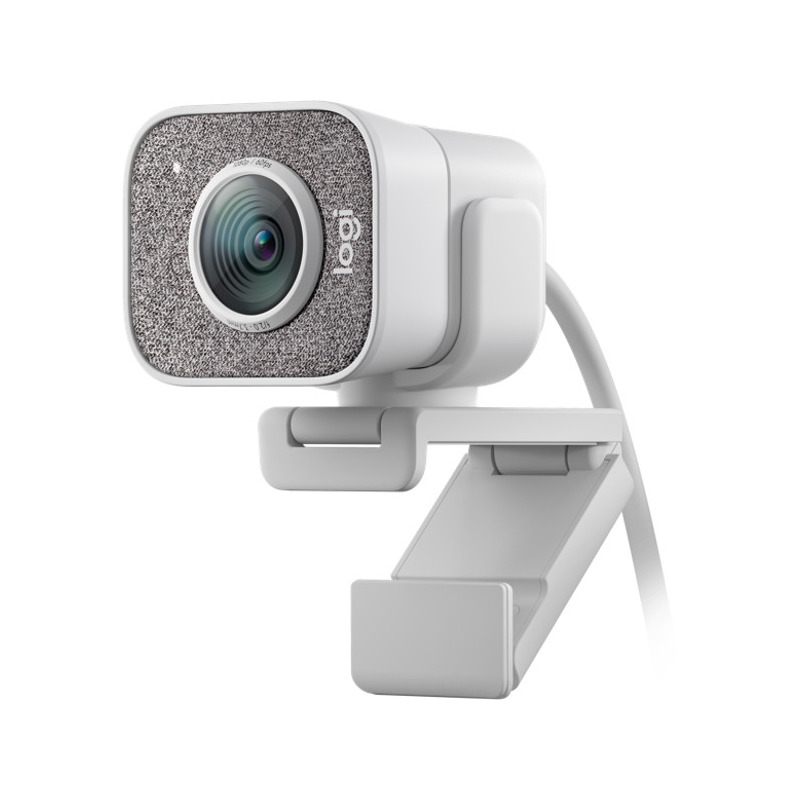
\includegraphics[width=0.3\textwidth]{webcam.jpg}
    \caption{Exemplu de webcam ce poate fi montat pe monitorul unui calculator. Imagine preluată de pe \href{https://www.pcgarage.ro/camere-web/logitech/streamcam-off-white/}{PC Garage}}
\end{figure}

Lucrarea de față ia în considerare popularitatea acestui webcam și propune o soluție pentru a putea folosi parțial un calculator fără ajutorul mâinilor.
O mare parte din interacțiunea dintre om și calculator se petrece \emph{prin intermediul mouse-ului}, așadar m-am concentrat pe simularea comportamentului acestuia \emph{folosind doar caracteristici ale feței}.
Ideea de bază constă în a prelua imagini ale utilizatorului de la webcam și, pe baza trăsăturilor faciale, de a simula funcționalități ale acestuia, spre exemplu de a muta cursorul în direcția în care privește utilizatorul.
Exemplul cel din urmă este cunoscut în litera științifică drept \emph{``Urmărirea ochilor''} (din engleză, \emph{``Eye tracking''}) și problema poate fi abordată prin tehnici de \emph{Învățare Automată}, o ramură a \emph{Inteligenței Artificiale}.

\begin{figure}[h]
    \centering
    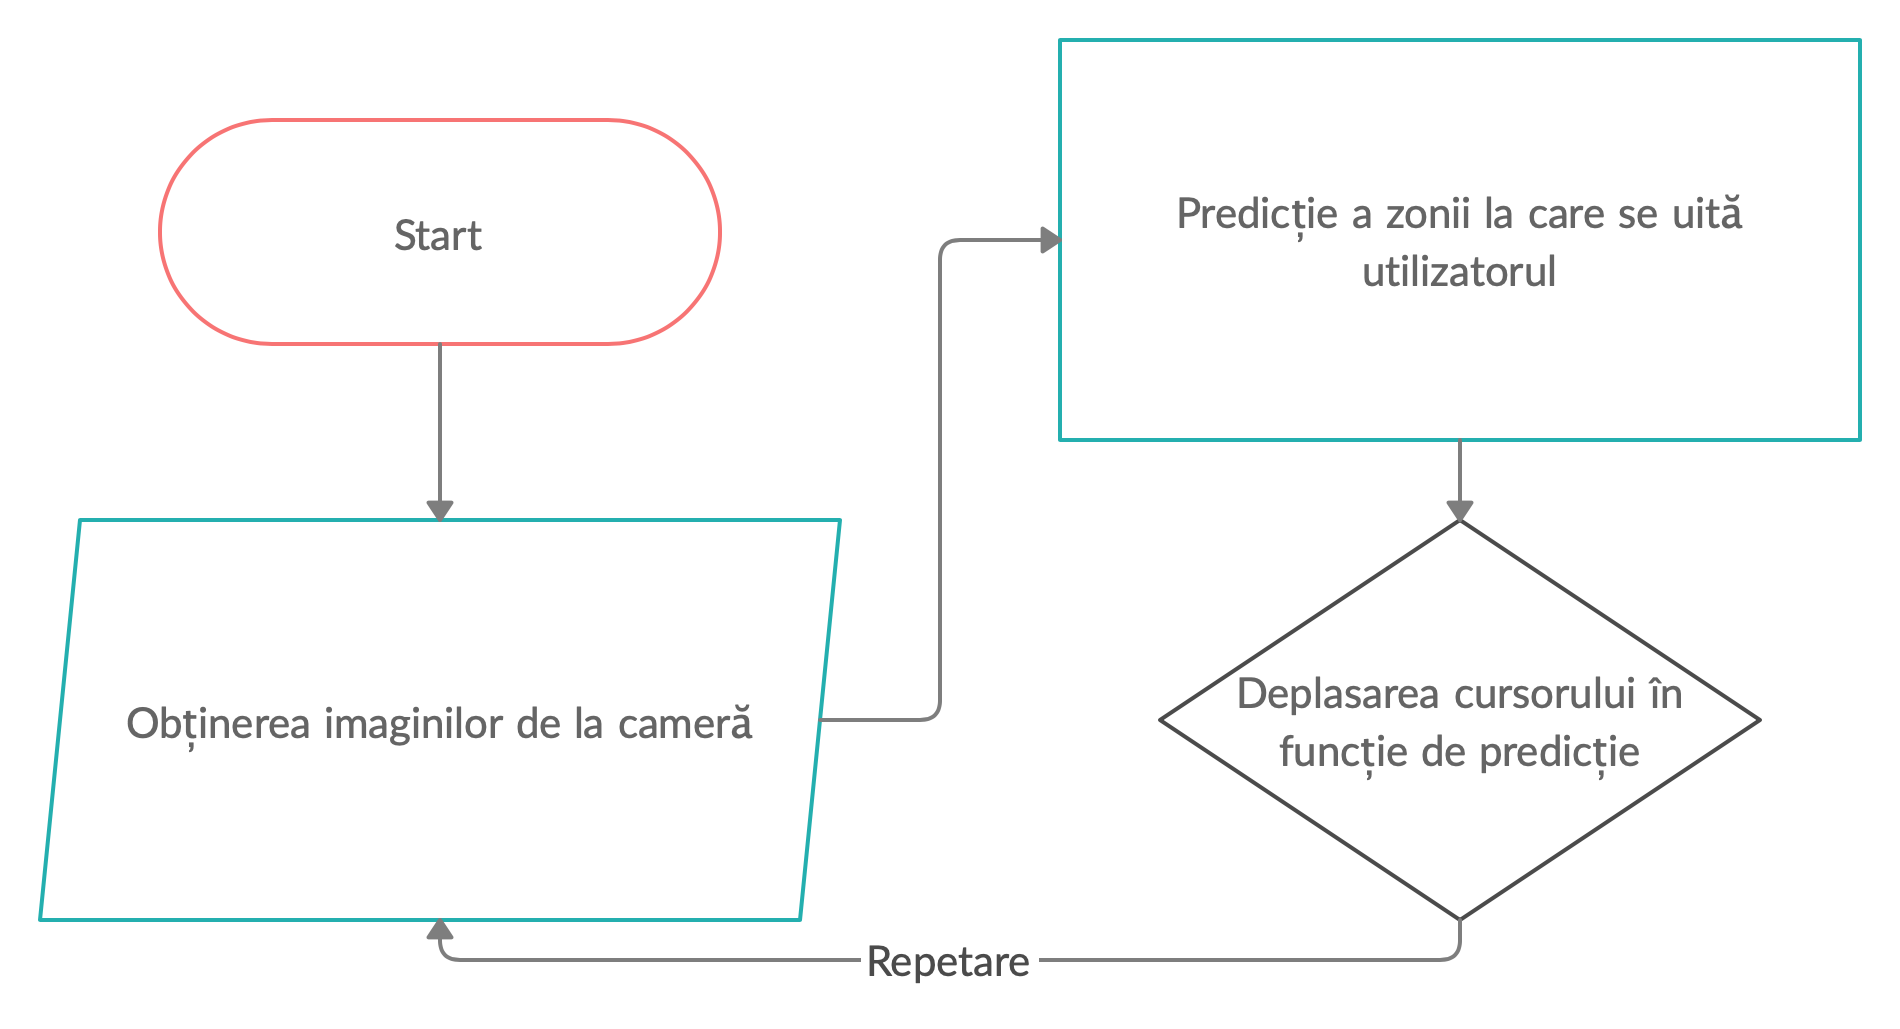
\includegraphics[width=\textwidth]{idee.png}
    \caption{Schemă generală pentru deplasarea cursorului}
\end{figure}

Această idee nu este nouă și există deja soluții pentru această problemă, bazate pe aceeași idee.
Totuși, cele mai multe dintre ele sunt create ori doar pentru un anumit sistem de operare (în acest caz, Windows), ori nu sunt gratuite și au un cost atașat semnificativ, sau chiar necesită componente hardware adiționale.

\emph{Camera Mouse}\footnote{\url{http://www.cameramouse.org}} este o propunere viabilă care urmărește o porțiune fixată a feței (spre exemplu vârful nasului) și, când acea porțiune își schimbă poziția, se schimbă și poziția cursorului.
Pentru ca acest lucru să funcționeze, utilizatorul trebuie să efectueze mișcări ale capului.
Oferă și functionalități de simulare a apăsării pe butoanele mouse-ului, însă aplicația funcționează doar pentru sistemele care rulează Windows.
Printre alternative se mai găsesc \emph{IntelliGaze}\footnote{\url{https://www.intelligaze.com/en/}} și produse dezvoltate de \emph{Tobii Dynavox}\footnote{\url{https://www.tobiidynavox.com/software/windows-software/windows-control-2/}}, dar acestea necesită în primul rând hardware adițional, lucrează doar pentru sistemul de operare Windows și au și un cost atașat.

\section*{Motivație}
\addcontentsline{toc}{section}{Motivație}

Când a trebuit să mă decid asupra temei lucrării de licență, am luat în calcul doi factori cheie: viitoarea mea carieră profesională și utilitatea proiectului.
Mi-am dorit să lucrez la un proiect care mi-ar alimenta interesul în Inteligența Artificială și care mi-ar oferi șansa de a aplica cercetarea pe care aș face-o în acest domeniu.
Mai mult, mi-am dorit de asemenea să am și o abordare practică asupra lucrării, astfel încât să construiesc ceva ce ar fi folositor.

Cât despre Inteligența Artificială, este inutil să-i subliniem importanța contemporană.
De la aplicabilitatea medicală, conducere/pilotare autonomă, agricultură inteligentă până la frigidere inteligente care-ți spun când ai rămas fără lapte, Inteligența Artificială este larg răspândită și extinderea ei nu se va opri prea curând.
Pentru mine, acesta este un motiv în plus pentru a o studia și a o înțelege mai bine, mai ales că o găsim integrată în viața noastră de zi cu zi.

\section*{Obiective}
\addcontentsline{toc}{section}{Obiective}
Cel mai important obiectiv al acestei lucrări de licență este înțelegerea și aplicarea cu succes a cunoștințelor și a noțiunilor dobândite ca student al Facultății de Informatică, Iași.
Toate noțiunile teoretice și practice acumulate trebuie să se regăsească într-o combinație armonioasă pentru a putea permite dezvoltarea unui software de calitate.
Am încercat, în acest sens, să țin cont de concepte precum principii de \emph{software design} (spre exemplu principiile de programare \emph{SOLID}), de \emph{design patterns} precum \emph{MVP}, de concepte de analizare a complexității timp/spațiu, de noțiuni legate de învățarea automată (spre exemplu tratarea \emph{overfitting-ului}) și altele.

Obiectivul principal al aplicației este acela de a simula folosirea unui mouse doar prin gesturi ale feței.
Prima parte a obiectivului se traduce în urmărirea ochilor utilizatorului, pentru a ști în ce direcție să deplasăm cursorul, și este partea pe care se concentrează cel mai mult această lucrare.
Având această capacitate, aplicația trebuie apoi să pună la dispoziție utilizatorului modalități de a simula, prin folosirea feței, cele mai importante funcționalități ale unui mouse:
\begin{itemize}
    \item mișcarea cursorului
    \item apăsarea butonului stâng
    \item apăsarea butonului drept\footnote{Aceste funcționalități mai sunt denumite uzual și ``click stânga/dreapta''}
\end{itemize}

\begin{figure}[h]
    \centering
    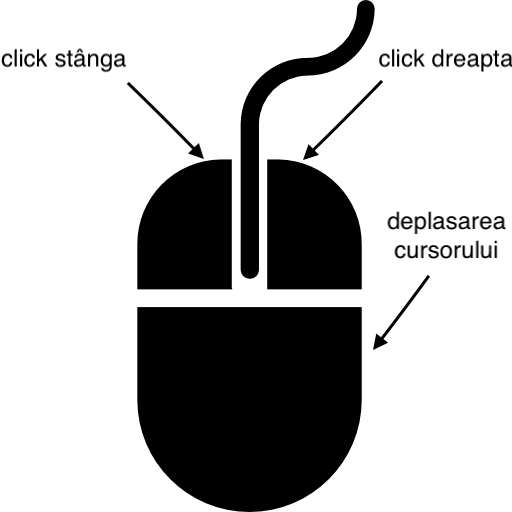
\includegraphics[width=0.5\textwidth]{mouse.png}
    \caption{Funcționalități principale ale unui mouse. Imagine preluată și adaptată de pe \href{https://www.flaticon.com}{Flaticon}, autor: \href{https://www.flaticon.com/authors/kiranshastry}{Kiranshastry}}
\end{figure}

% \section*{Metodologie}
% \addcontentsline{toc}{section}{Metodologie}

\section*{Descriere sumară a soluției}
\addcontentsline{toc}{section}{Descriere sumară a soluției}

Fața umană poate fi analizată pe baza mai multor \emph{repere faciale}.
Acestea sunt reprezentate prin anumite puncte de pe față precum centrul ochiului, centrul nasului, centrul buzei superioare etc.
Cunoscând acestea, putem delimita zone ale feței precum un singur ochi.
În figura de mai jos\ref{figure:facial-landmarks}, ochiul stâng al unei persoane este delimitat de înfășurătoarea convexă a punctelor cu indicii $[43, 48]$.

\begin{figure}[h]
    \centering
    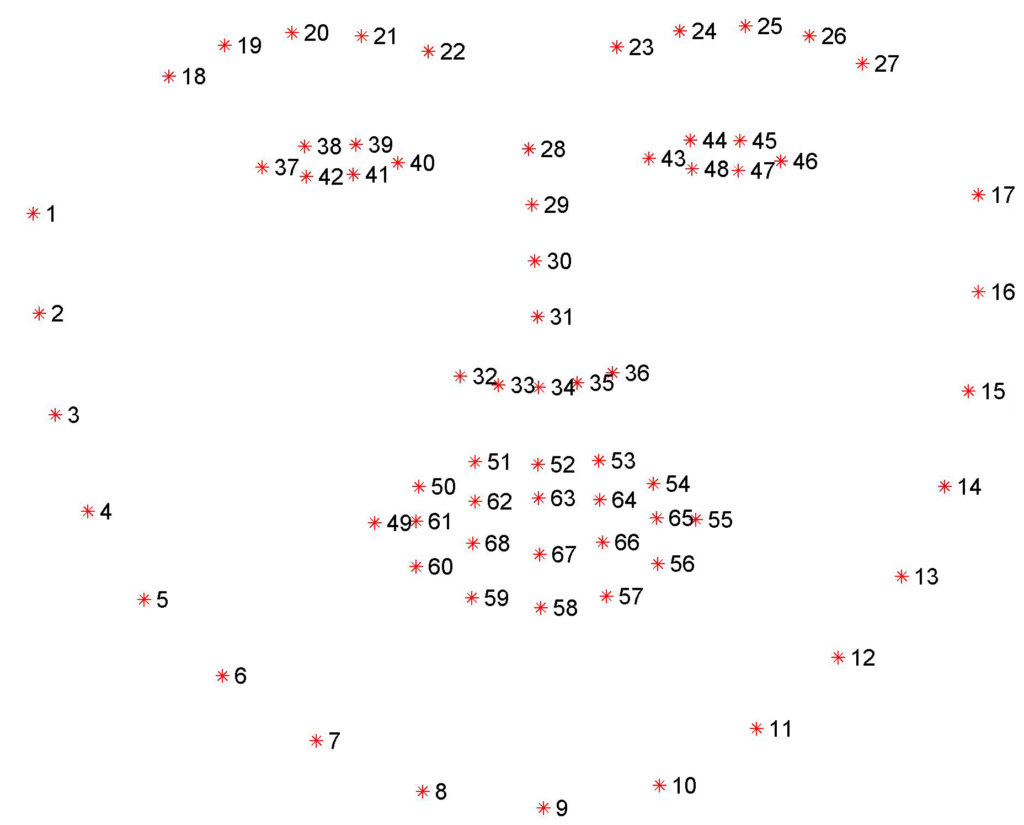
\includegraphics[width=0.49\textwidth]{facial_landmarks_1.jpg}
    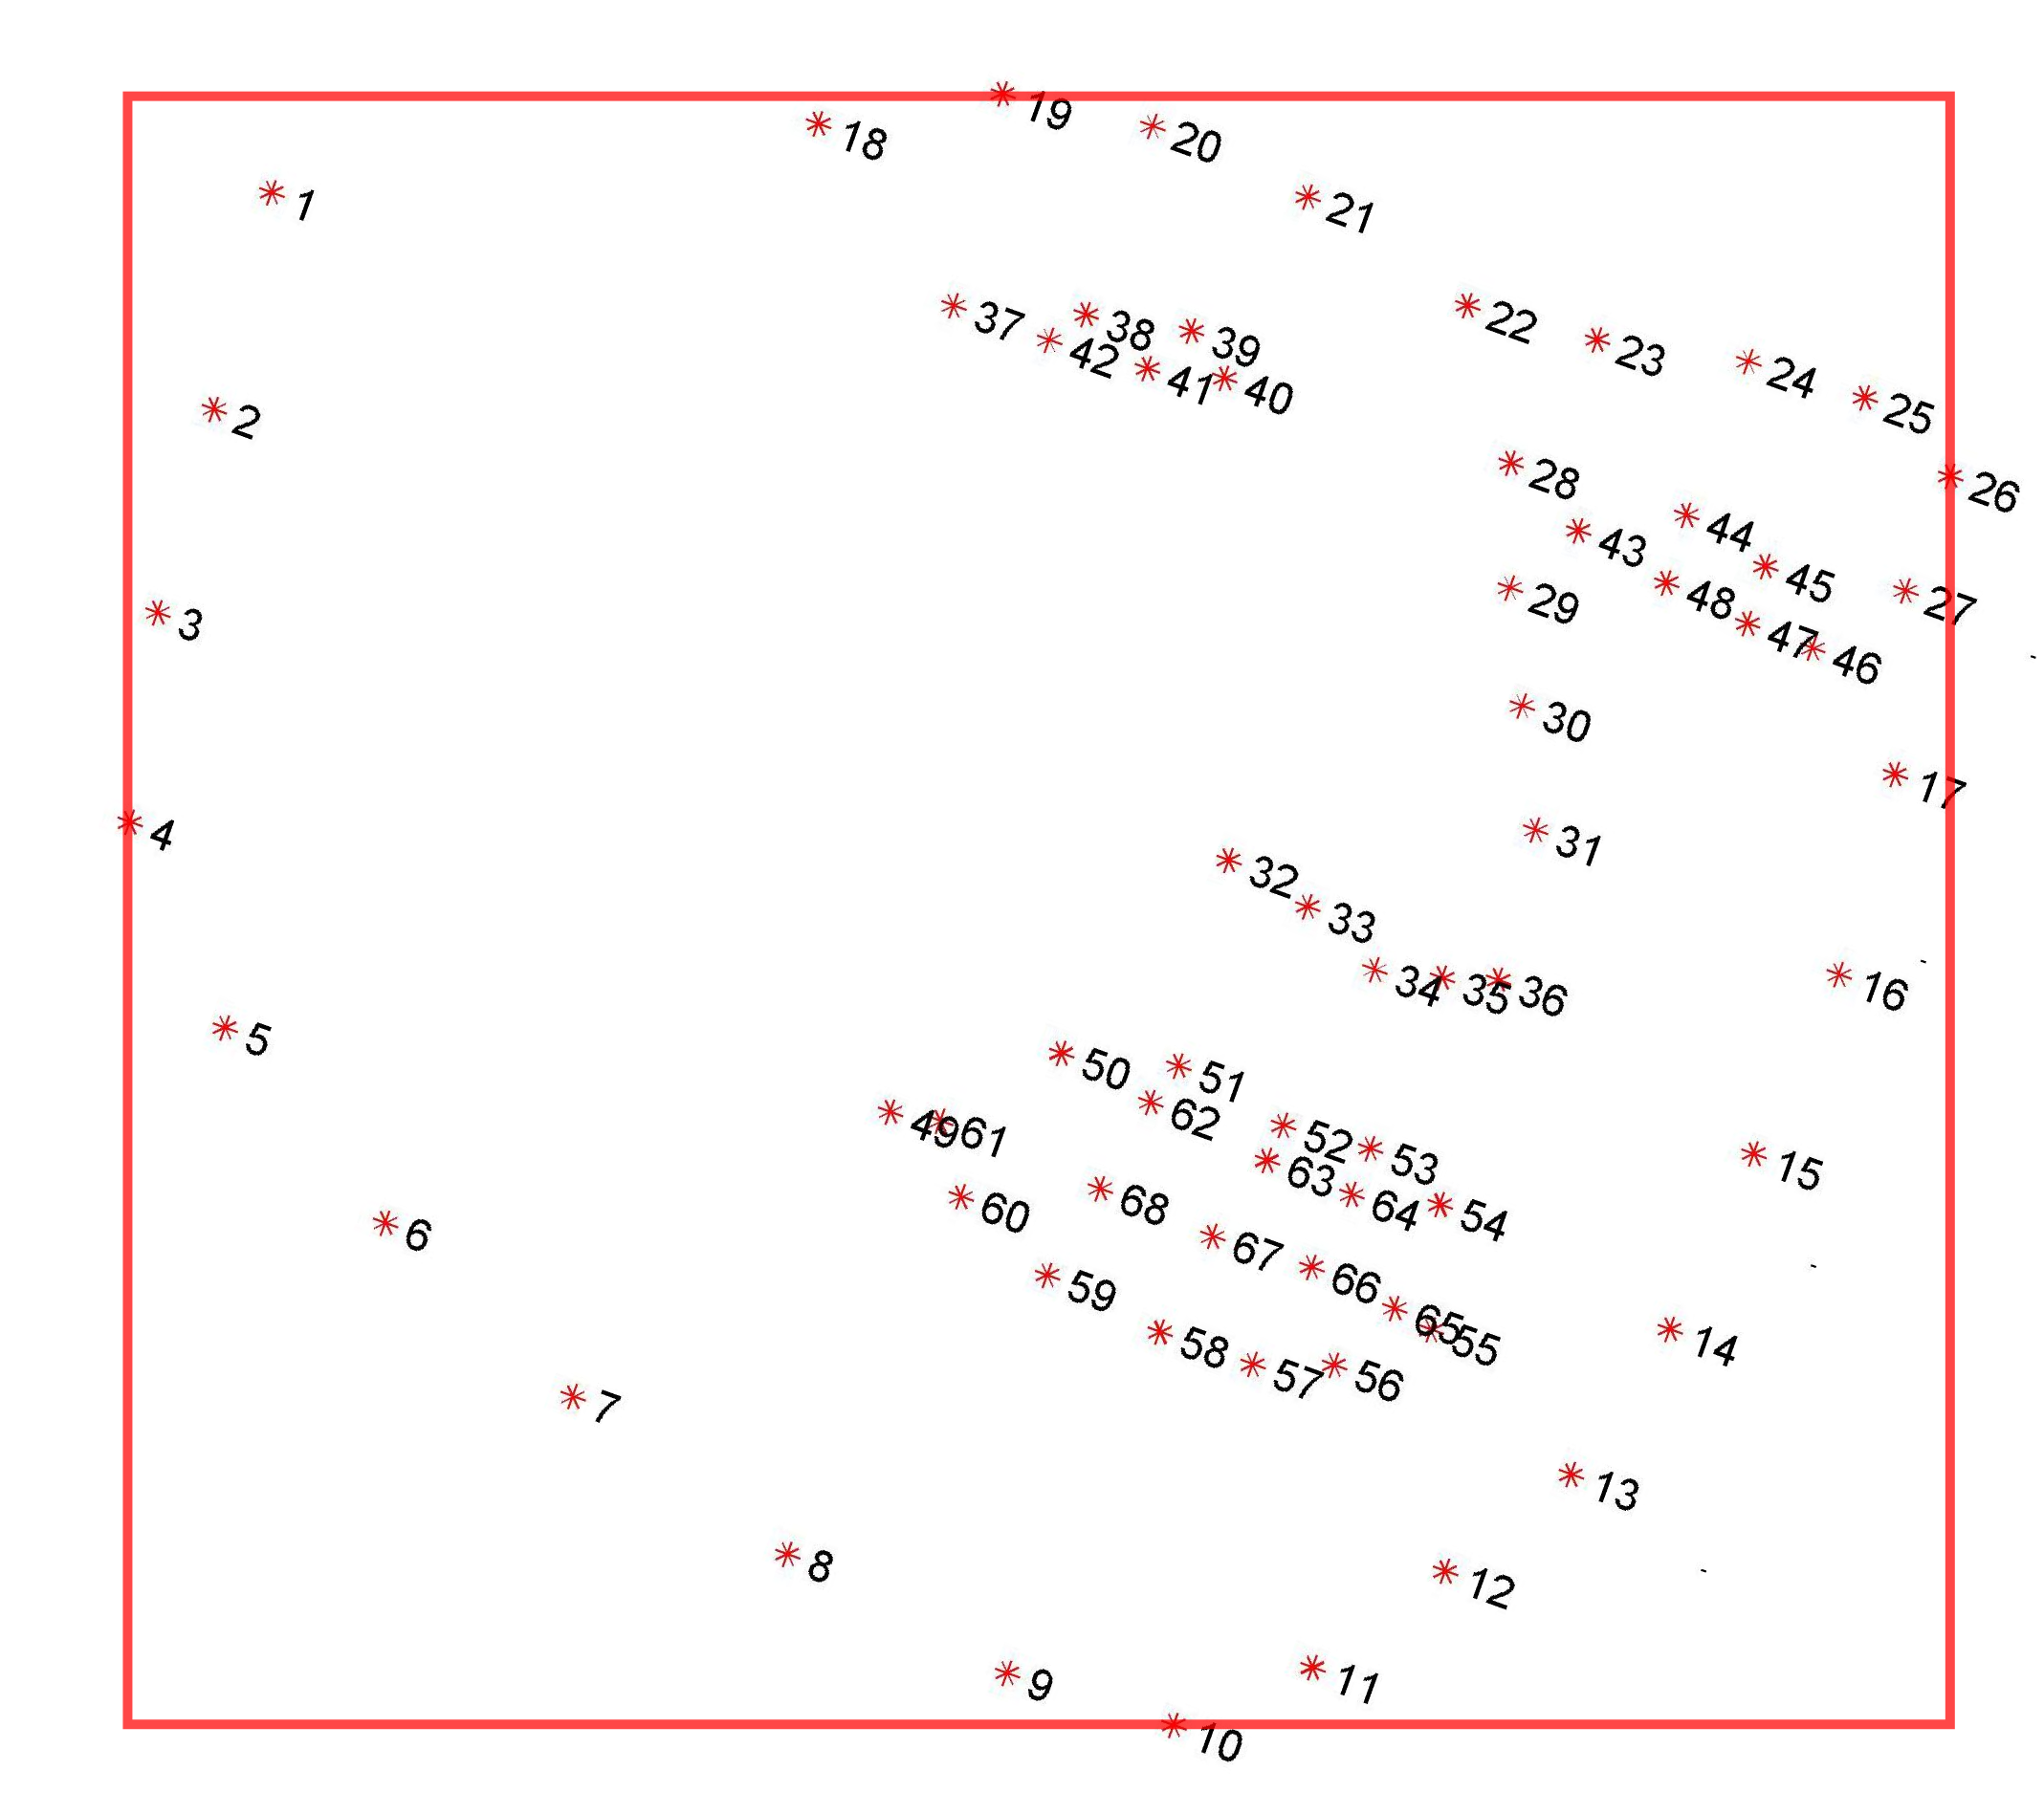
\includegraphics[width=0.49\textwidth]{facial_landmarks_2.png}
    \caption{Repere faciale. Imagini preluate de aici: \url{https://ibug.doc.ic.ac.uk/resources/300-W/}}
    \label{figure:facial-landmarks}
\end{figure}

Folosind anumiți algoritmi deja existenți am detectat aceste puncte faciale din imagini ale utilizatorului aplicației (în acest caz, imagini cu mine însumi) iar apoi am extras regiuni dreptunghiulare care conțineau fie întreaga față, fie ochii persoanei.
Apoi am etichetat aceste imagini decupate cu coordonatele punctelor de pe ecran pe care le privea utilizatorul în fiecare imagine și am dezvoltat un model matematic care poate calcula zona ecranului pe care o privește utilizatorul.

Mai departe am făcut uz de restul reperelor faciale pentru a putea atinge obiectivele prezentate mai devreme.
Fiind capabilă să urmărească ochii, aplicația trebuie și să poată deplasa cursorul, dar într-un mod controlat, care să nu deranjeze privirea normală a ecranului (nu întotdeauna când privim ecranul dorim să deplasăm cursorul).
Astfel, deplasarea cursorului se realizează doar în momentul în care distanța dintre buza superioară și cea inferioară este nenulă și reprezintă un anumit procent din distanța dintre extremitățile buzelor (care coincid).
În termeni mai populari și mai simpli, relația se traduce prin gestul de deschidere a gurii.

Pentru apăsarea butoanelor am avut o abordare similară.
Prin închiderea ochiului stâng pentru o anumită perioadă de timp se realizează apăsarea butonului stâng.
Analog, apăsarea butonului drept se realizează similar.
Aceste lucruri au dus la îndeplinirea obiectivelor prezentate mai devreme, întrucât aplicația poate fi minipulată exclusiv prin fața utilizatorului.

\section*{Structura lucrării}
\addcontentsline{toc}{section}{Structura lucrării}
În primul capitol am prezentat principala problemă pe care o analizează această lucrare, și anume urmărirea ochilor (\emph{eye tracking}).
Este prezentată de asemenea strategia pe care am abordat-o spre rezolvarea acestei probleme.

Următorul capitol prezintă soluția propusă împreună cu limitele și constrângerile acesteia.
Am ilustrat structura acesteia, componentele principale și șablonul arhitectural (\emph{design pattern-ul}) folosit pentru a ghida dezvoltarea aplicației.

Capitolele 3, 4 și 5 urmăresc pașii luați în rezolvarea unei probleme de învățare automată.
Am început cu modul în care am obținut datele de antrenament, modul în care le-am procesat iar apoi am continuat cu prezentarea modului de antrenare și de dezvoltare a arhitecturilor de învățare profundă pe care le-am folosit.
Capitolul 5 prezintă modul în care am folosit predicțiile de urmărire a ochilor în combinație cu repere faciale pentru a simula funcționalitatea unui mouse.

În cele din urmă, capitolul 6 ilustrează un experiment pe care l-am făcut pentru identificarea reperelor faciale.
Acesta m-a ajutat la o înțelegere mai bună a modului în care reperele faciale sunt identificate.

